\documentclass[11pt, a4paper]{article}  %(或book)
%\documentclass{emulateapj}
%\usepackage[Lenny]{fncychap}  %(章节的格式设置)
\usepackage{titlesec}
\titleformat{\section}{\Large\bfseries}{\thesection}{1em}{}
\titleformat{\subsection}{\large\bfseries}{\thesubsection}{1em}{}
% \titleformat{\section}{标题的格式,包括字体,字体大小,加粗}{标题序号,\thesection是数字,可自定义如“Di \thesection Zhang”}{标题序号与标题文字之间空格的大小,用pt或em,不能省}{标题文字大小,用\large等,可缺省}
\usepackage{amsmath}
\usepackage{amssymb}
\usepackage{float}
\usepackage{natbib}
\usepackage{color}
\usepackage{mathrsfs}
\usepackage{graphicx}
\usepackage{CJK}  %(CJK宏包,也可以写成\usepackage{CJKutf8})
\usepackage{setspace}
\usepackage{graphicx}
\usepackage{multirow}
\usepackage{tabularx}
\usepackage{indentfirst} % indent at each head of graphy
\usepackage{subfigure} % 在\begin{figure}环境下插入横排并列的子图
\usepackage{multicol} % 部分页面的文字分栏设置(不适用于图片和表格)
\usepackage[top=3cm, bottom=3cm, left=2cm, right=2cm]{geometry}  %(边距)
% \newgeometry{left=..} % 会另起一新页,然后从该新页开始使用新的边距,直到遇到 \restoregeometry 为止

\begin{document}
\begin{CJK}{UTF8}{gbsn}  %(用UTF8编码,否则可能乱码,一定要3个{}都有)
\nocite{*}
\setlength{\parskip}{6pt}  % 设置标题上下的间距(\setlenght要在\begin{document}之后才有效果)
\setlength{\baselineskip}{20pt} % 设置每一行的行距

%\begin{figure}[htbp]/[H]
%%\center
%\includegraphics[width=xxcm]{figure.eps}
%\subfigure{ \includegraphics[width=xxcm]{test1.eps} } % 注意\subfigure后有{}
%\subfigure{ \includegraphics[width=xxcm]{test2.eps} } % 插入横排并列图片
%\subfigure{ \includegraphics[width=xxcm]{test3.eps} }
%\caption{Explain of figure}
%\label{fig:figurelabel}
%\end{figure}

%\begin{table}[htbp]/[H]
%\center
%\begin{tabular}{llcccr}  % number of columns, c->center, l->left, r->right
%\hline\hline  % \hline->horizontal line
%& Mass($M_{\text{sun}}$) & Radius(km) \\  % use "&" to align, "$$" to insert formula, "\\" to break the row
%\label{tab:tablelabel}
%\end{tabular}
%\end{table}

%\begin{eqnarray}
%	f(t) = \left\{ \begin{aligned}
%			a+bt & \, \quad t<0 \\
%			0    & \, \quad t \ge 0
%\end{aligned} \right.
%\end{eqnarray}


\title{\huge 高斯模糊/平滑/滤波\\Gaussian Blur/Smoothing/Filter \bf }

\author{Qizhi Huang}
\date{\today}
\maketitle
%%%%%%%%%%%%%%% Begin %%%%%%%%%%%%%%%



用$\mu=0$的高斯函数
\begin{equation}
	F(x) = \frac{1}{\sigma \sqrt{2\pi}} \, e^{-\frac{x^2}{2\sigma^2}}
\end{equation}
对数据进行平滑,可以有效地压低数据中的高斯噪声。

原数据:$\sigma_{\text{in}}$,高斯滤波器:$\sigma_{\text{filter}}$,平滑数据:$\sigma_{\text{out}}$

\begin{equation}
	\sigma_{\text{out}} \approx \frac{\sigma_{\text{in}}}{\sqrt{\sigma_{\text{filter}} \cdot 2\sqrt{\pi}}}
\label{eq:sr}
\end{equation}

Equation (\ref{eq:sr}) above is right (checked by python program). Figure below is wrong (also wiki: \\
https://en.wikipedia.org/wiki/Gaussian\_blur)

\begin{figure}[H]
\center
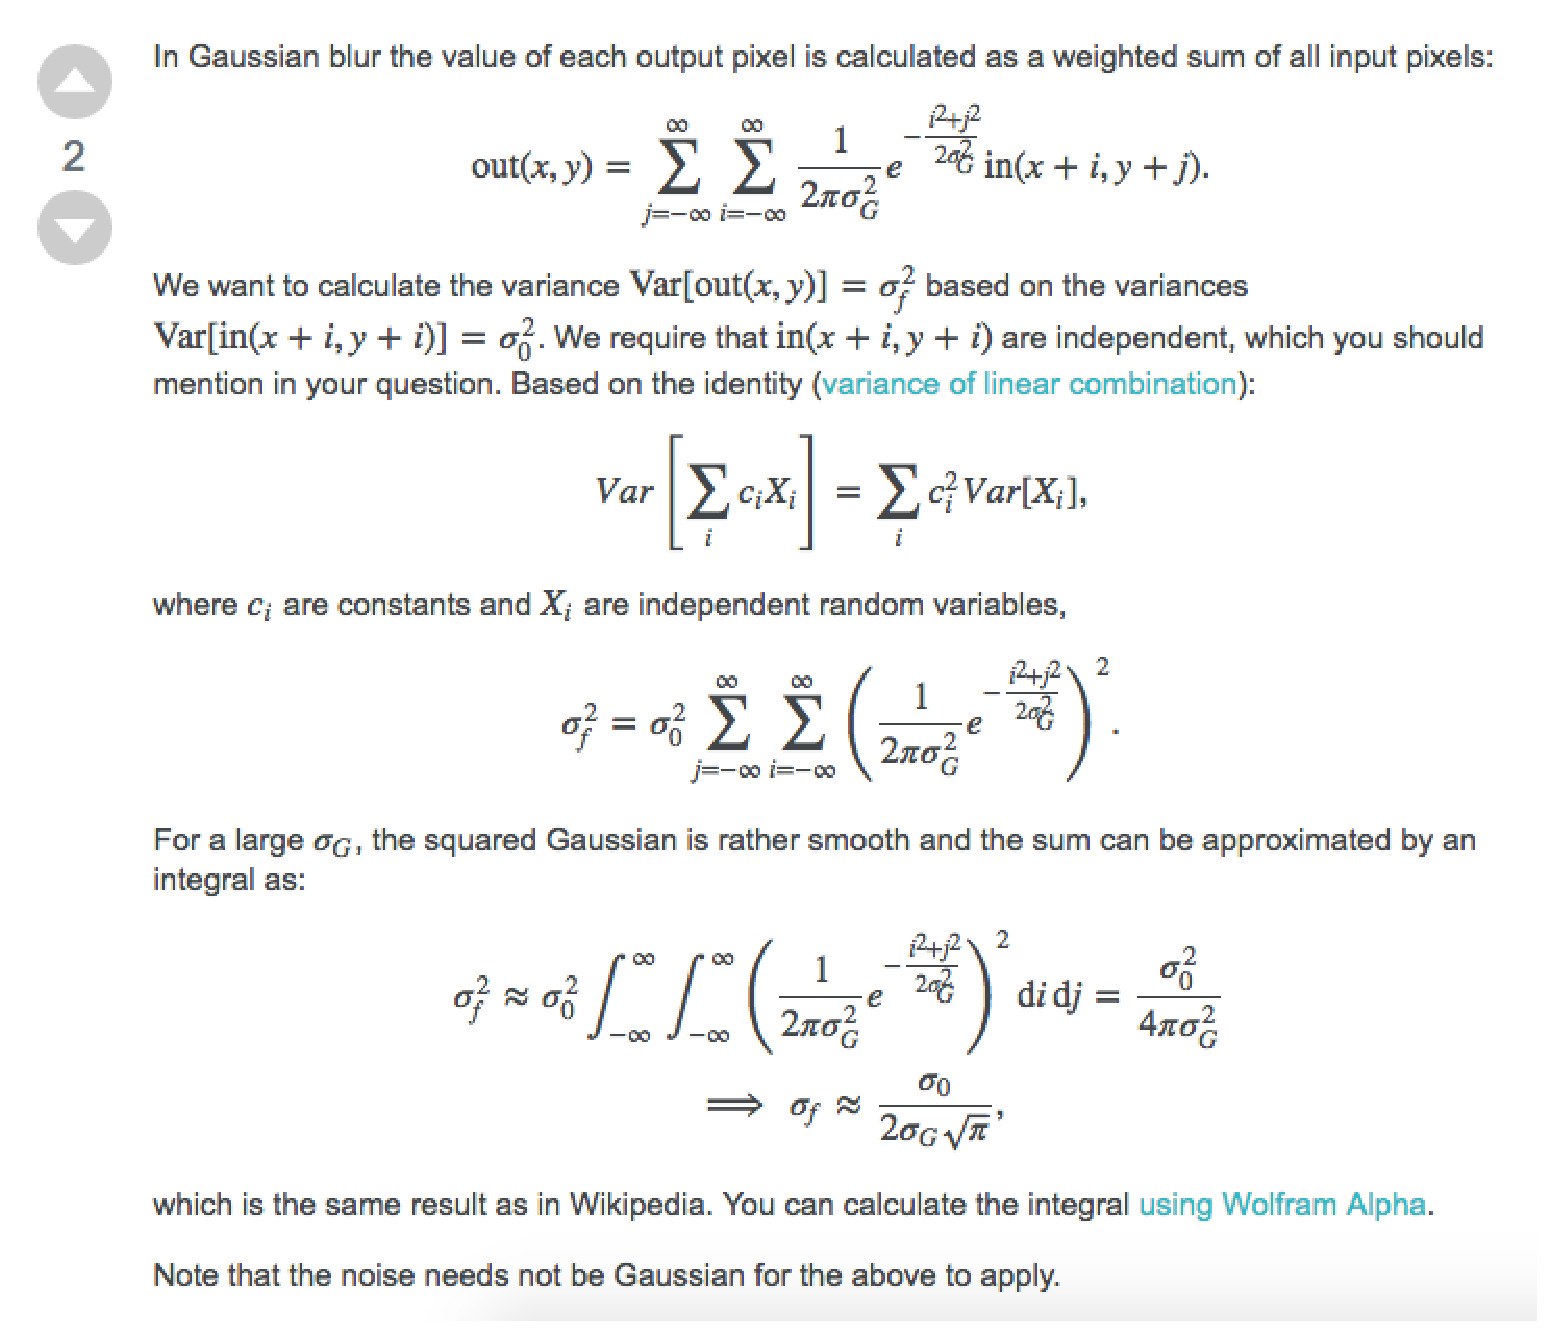
\includegraphics[width=11.5cm]{gaussian_blur-smoothing-filter.eps}
\end{figure}



%%%%%%%%%%%%%%% End %%%%%%%%%%%%%%%
\end{CJK}
\end{document}
